\NeedsTeXFormat{LaTeX2e}
%\PassOptionsToClass{handout}{beamer}
\documentclass{beamer}
\usepackage{beamerPack}
\usepackage{setspace}
\usepackage{markdown}
\usepackage[05]{../lecture}
\subtitle{プログラミング的思考cntd.}
\begin{document}

\begin{frame}[fragile]{}
\titlepage
\end{frame}

\section{Algorithm design}		%%%%%%%%
\subsection{}

\begin{frame}[fragile]{問題解決の枠組み}{}
\begin{enumerate}\itemsep8pt
\item 問題の解法をアルゴリズム化する
\begin{align*}
アルゴリズム = & 前処理? 相似問題^{+} 後処理?
\end{align*}
\item (要求を満たすまで無駄を省く)
\item プログラムとして実装する
\item (要求を満たすまで高速化する)
\end{enumerate}
\end{frame}

\begin{frame}[fragile]{問題1.0}{文章題=論理的思考力+アルゴリズム}
\begin{tikzpicture}[overlay, xshift=0.5\textwidth,yshift=-0.33\textheight]
\node at (0,0) {\pgfimage[width=1.1\pagewidth]{shuttle.jpg}};
\end{tikzpicture}
\begin{spacing}{1.25}
\textcolor{white}{
観光用スペースシャトルが高度100キロメートルからツアーを開始します。\\
乗客は1分ごとに次の1分間上昇するか、下降するかを決めることができます。どちらも1分でちょうど1キロ上昇するか下降します。\\
30分後(30回の進路変更後)に元の高度に戻ってこなければならないとすると、飛行経路は何通りあるでしょう。
}
\end{spacing}
\end{frame}

\begin{frame}[fragile]{問題1.1}{}
\begin{tikzpicture}[overlay, xshift=0.5\textwidth,yshift=-0.28\textheight]
\node at (0,-1) {\pgfimage[width=0.55\pagewidth]{smalltalk.jpg}};
\end{tikzpicture}

\begin{spacing}{1.25}
観光用飛行船が高度5キロメートルからツアーを開始します。\\
乗客は1分ごとに次の1分間上昇するか、下降するかを決めることができます。どちらも1分でちょうど1キロ上昇するか下降します。\\
30分後(30回の進路変更後)に元の高度に戻ってこなければならないとすると、飛行経路は何通りあるでしょう。\\
高度0キロメートルで墜落します。
\end{spacing}
\end{frame}

\begin{frame}[fragile]{問題1.2}{}
あなたは\textcolor{blue}{Aブロック}でお客を拾ったタクシードライバーです。お客は\textcolor{red}{Bブロック}に行こうとしています。
リアルタイム混雑情報サービスはブロック内移動時間を以下のように表示しています。
最短で何分あればBブロックに到着できるでしょう。
どのブロックも下から上または左から右へ一方通行でつながっています。

\begin{center}
\scalebox{0.25}{
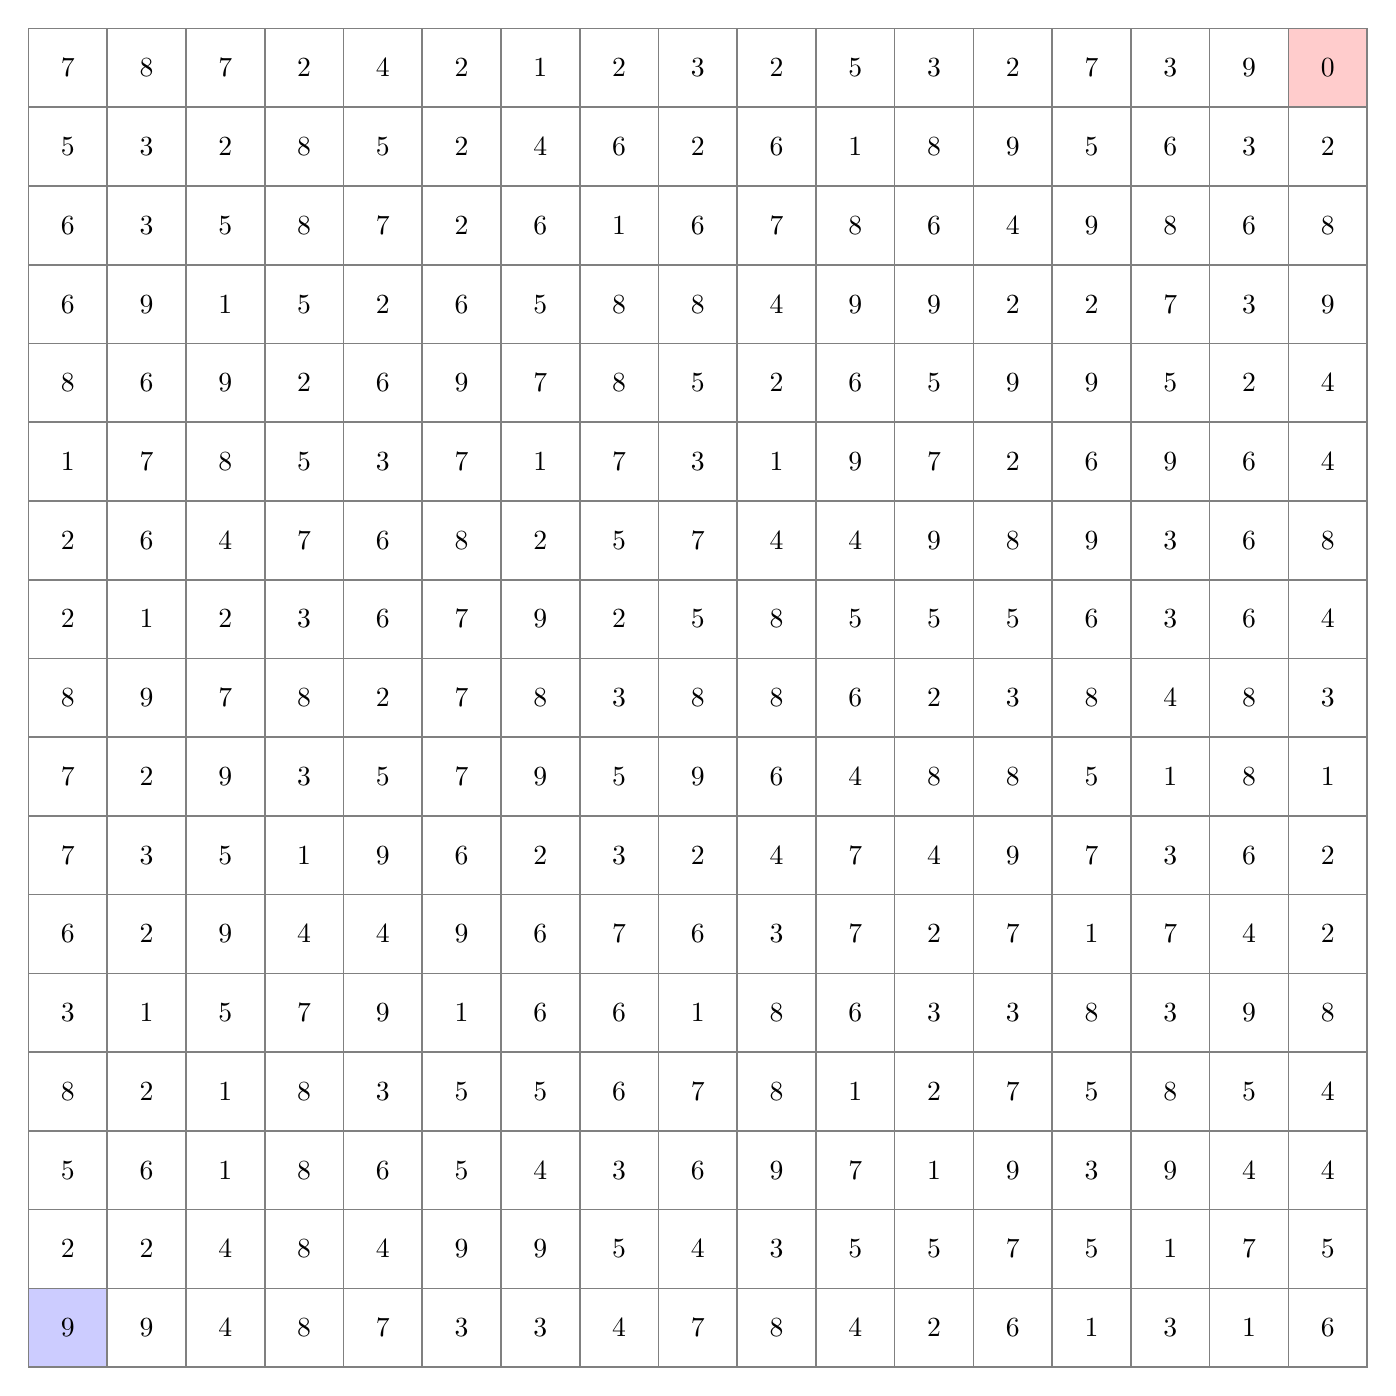
\begin{tikzpicture}[cell/.style = {rectangle,draw=gray,semithick,minimum size=1cm,outer sep=0mm}]
\node[cell,fill=blue!20] at (0,0) {};
\node[cell,fill=red!20] at (16,16) {};
    \foreach \i [count=\j from 0] in {9,9,4,8,7,3,3,4,7,8,4,2,6,1,3,1,6} \node[cell] at (\j, 0) {$\i$};
    \foreach \i [count=\j from 0] in {2,2,4,8,4,9,9,5,4,3,5,5,7,5,1,7,5} \node[cell] at (\j, 1) {$\i$};
    \foreach \i [count=\j from 0] in {5,6,1,8,6,5,4,3,6,9,7,1,9,3,9,4,4} \node[cell] at (\j, 2) {$\i$};
    \foreach \i [count=\j from 0] in {8,2,1,8,3,5,5,6,7,8,1,2,7,5,8,5,4} \node[cell] at (\j, 3) {$\i$};
    \foreach \i [count=\j from 0] in {3,1,5,7,9,1,6,6,1,8,6,3,3,8,3,9,8} \node[cell] at (\j, 4) {$\i$};
    \foreach \i [count=\j from 0] in {6,2,9,4,4,9,6,7,6,3,7,2,7,1,7,4,2} \node[cell] at (\j, 5) {$\i$};
    \foreach \i [count=\j from 0] in {7,3,5,1,9,6,2,3,2,4,7,4,9,7,3,6,2} \node[cell] at (\j, 6) {$\i$};
    \foreach \i [count=\j from 0] in {7,2,9,3,5,7,9,5,9,6,4,8,8,5,1,8,1} \node[cell] at (\j, 7) {$\i$};
    \foreach \i [count=\j from 0] in {8,9,7,8,2,7,8,3,8,8,6,2,3,8,4,8,3} \node[cell] at (\j, 8) {$\i$};
    \foreach \i [count=\j from 0] in {2,1,2,3,6,7,9,2,5,8,5,5,5,6,3,6,4} \node[cell] at (\j, 9) {$\i$};
    \foreach \i [count=\j from 0] in {2,6,4,7,6,8,2,5,7,4,4,9,8,9,3,6,8} \node[cell] at (\j, 10) {$\i$};
    \foreach \i [count=\j from 0] in {1,7,8,5,3,7,1,7,3,1,9,7,2,6,9,6,4} \node[cell] at (\j, 11) {$\i$};
    \foreach \i [count=\j from 0] in {8,6,9,2,6,9,7,8,5,2,6,5,9,9,5,2,4} \node[cell] at (\j, 12) {$\i$};
    \foreach \i [count=\j from 0] in {6,9,1,5,2,6,5,8,8,4,9,9,2,2,7,3,9} \node[cell] at (\j, 13) {$\i$};
    \foreach \i [count=\j from 0] in {6,3,5,8,7,2,6,1,6,7,8,6,4,9,8,6,8} \node[cell] at (\j, 14) {$\i$};
    \foreach \i [count=\j from 0] in {5,3,2,8,5,2,4,6,2,6,1,8,9,5,6,3,2} \node[cell] at (\j, 15) {$\i$};
    \foreach \i [count=\j from 0] in {7,8,7,2,4,2,1,2,3,2,5,3,2,7,3,9,0} \node[cell] at (\j, 16) {$\i$};
\end{tikzpicture}
}
\end{center}
\end{frame}

\begin{frame}[fragile]{配布ファイル}{toa04-p1.2-routes.txt}
\begin{codeof}{language=c}{行が列より先:j, i = N}
 0, 0 = 9
 0, 1 = 9
 0, 2 = 4
 0, 3 = 8
 0, 4 = 7
...
 1, 0 = 2
 1, 1 = 2
 1, 2 = 4
 1, 3 = 8
...
 2, 0 = 5
\end{codeof}

1行目の意味:座標$(0, 0)$のブロックを(どの方向であれ)通り抜けるには9分かかる。
従ってそこから座標$(1,0)$や$(0,1)$のブロックにたどり着くには9分が必要。
\end{frame}

\begin{frame}[fragile]{分解、組み合わせ、抽象化}{問題1.0と問題1.2は別問題か?}
\begin{itemize}\itemsep20pt
\item 問題1.0
\begin{enumerate}%\itemsep8pt
\item 再帰して
\item 再帰して
\item 組み合わせ:\texttt{+}を投入
\end{enumerate}
\item 問題1.2
\begin{enumerate}%\itemsep8pt
\item 再帰して
\item 再帰して
\item 組み合わせ:\texttt{min}を投入
\end{enumerate}
\end{itemize}

\vfill
両者は同じ
\end{frame}

\begin{frame}[fragile]{問題1.2.1}{}
あなたは\textcolor{blue}{Aブロック}でお客を拾ったタクシードライバーです。お客は\textcolor{red}{Bブロック}に行こうとしています。
RCISはそれぞれのブロック内移動時間を以下のように表示しています。
最短で何分あればBブロックに到着できるでしょう。
どのブロックも下から上、左から右、または左下から右上へ一方通行でつながっています。

\begin{center}
\scalebox{0.25}{
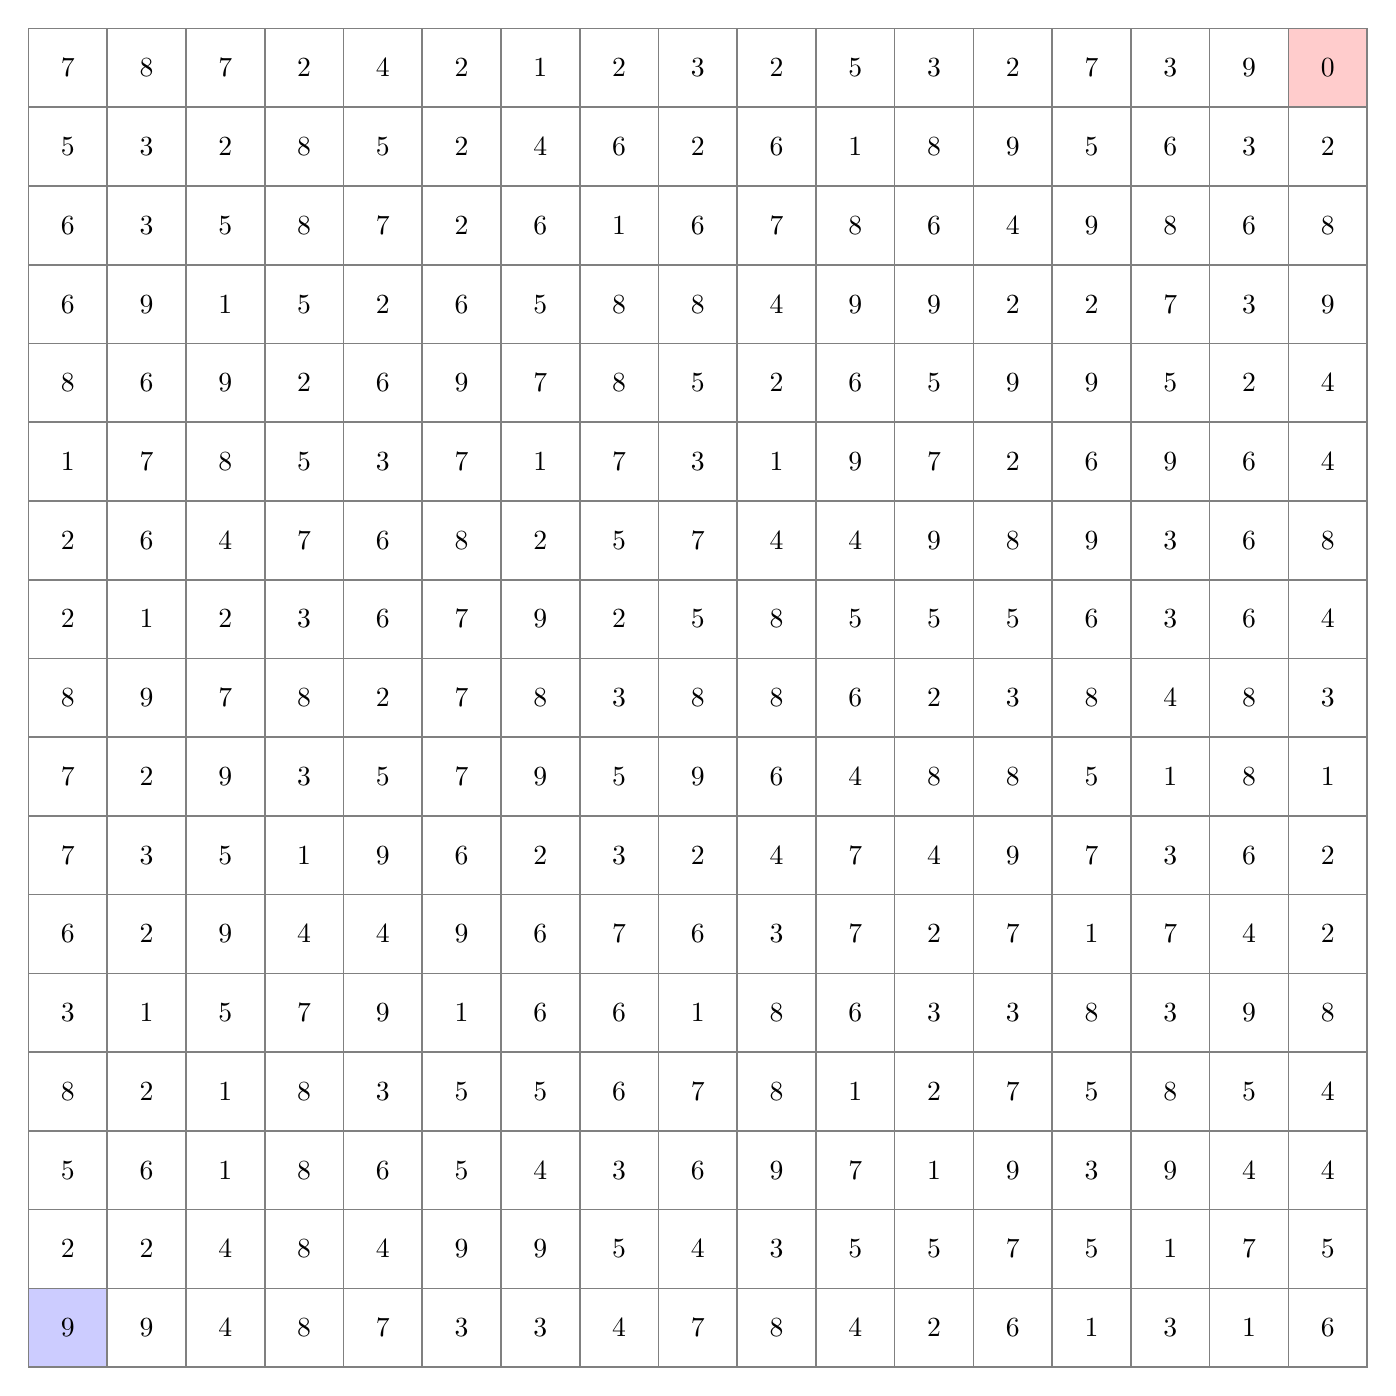
\begin{tikzpicture}[cell/.style = {rectangle,draw=gray,semithick,minimum size=1cm,outer sep=0mm}]
\node[cell,fill=blue!20] at (0,0) {};
\node[cell,fill=red!20] at (16,16) {};
    \foreach \i [count=\j from 0] in {9,9,4,8,7,3,3,4,7,8,4,2,6,1,3,1,6} \node[cell] at (\j, 0) {$\i$};
    \foreach \i [count=\j from 0] in {2,2,4,8,4,9,9,5,4,3,5,5,7,5,1,7,5} \node[cell] at (\j, 1) {$\i$};
    \foreach \i [count=\j from 0] in {5,6,1,8,6,5,4,3,6,9,7,1,9,3,9,4,4} \node[cell] at (\j, 2) {$\i$};
    \foreach \i [count=\j from 0] in {8,2,1,8,3,5,5,6,7,8,1,2,7,5,8,5,4} \node[cell] at (\j, 3) {$\i$};
    \foreach \i [count=\j from 0] in {3,1,5,7,9,1,6,6,1,8,6,3,3,8,3,9,8} \node[cell] at (\j, 4) {$\i$};
    \foreach \i [count=\j from 0] in {6,2,9,4,4,9,6,7,6,3,7,2,7,1,7,4,2} \node[cell] at (\j, 5) {$\i$};
    \foreach \i [count=\j from 0] in {7,3,5,1,9,6,2,3,2,4,7,4,9,7,3,6,2} \node[cell] at (\j, 6) {$\i$};
    \foreach \i [count=\j from 0] in {7,2,9,3,5,7,9,5,9,6,4,8,8,5,1,8,1} \node[cell] at (\j, 7) {$\i$};
    \foreach \i [count=\j from 0] in {8,9,7,8,2,7,8,3,8,8,6,2,3,8,4,8,3} \node[cell] at (\j, 8) {$\i$};
    \foreach \i [count=\j from 0] in {2,1,2,3,6,7,9,2,5,8,5,5,5,6,3,6,4} \node[cell] at (\j, 9) {$\i$};
    \foreach \i [count=\j from 0] in {2,6,4,7,6,8,2,5,7,4,4,9,8,9,3,6,8} \node[cell] at (\j, 10) {$\i$};
    \foreach \i [count=\j from 0] in {1,7,8,5,3,7,1,7,3,1,9,7,2,6,9,6,4} \node[cell] at (\j, 11) {$\i$};
    \foreach \i [count=\j from 0] in {8,6,9,2,6,9,7,8,5,2,6,5,9,9,5,2,4} \node[cell] at (\j, 12) {$\i$};
    \foreach \i [count=\j from 0] in {6,9,1,5,2,6,5,8,8,4,9,9,2,2,7,3,9} \node[cell] at (\j, 13) {$\i$};
    \foreach \i [count=\j from 0] in {6,3,5,8,7,2,6,1,6,7,8,6,4,9,8,6,8} \node[cell] at (\j, 14) {$\i$};
    \foreach \i [count=\j from 0] in {5,3,2,8,5,2,4,6,2,6,1,8,9,5,6,3,2} \node[cell] at (\j, 15) {$\i$};
    \foreach \i [count=\j from 0] in {7,8,7,2,4,2,1,2,3,2,5,3,2,7,3,9,0} \node[cell] at (\j, 16) {$\i$};
\end{tikzpicture}
}
\end{center}
\end{frame}

\begin{frame}[fragile]{問題1.3}{}
問題1.2を解くことで\textcolor{blue}{Aブロック}から各ブロックへの最短移動時間が以下に示す配列に格納された。
\textcolor{blue}{Aブロック}から\textcolor{red}{Bブロック}までの最短経路を次行の形式で出力せよ。
\begin{codeof}{}{}
(0,0) -> (1,0) -> ... -> (16,16)
\end{codeof}

\begin{center}
\scalebox{0.25}{
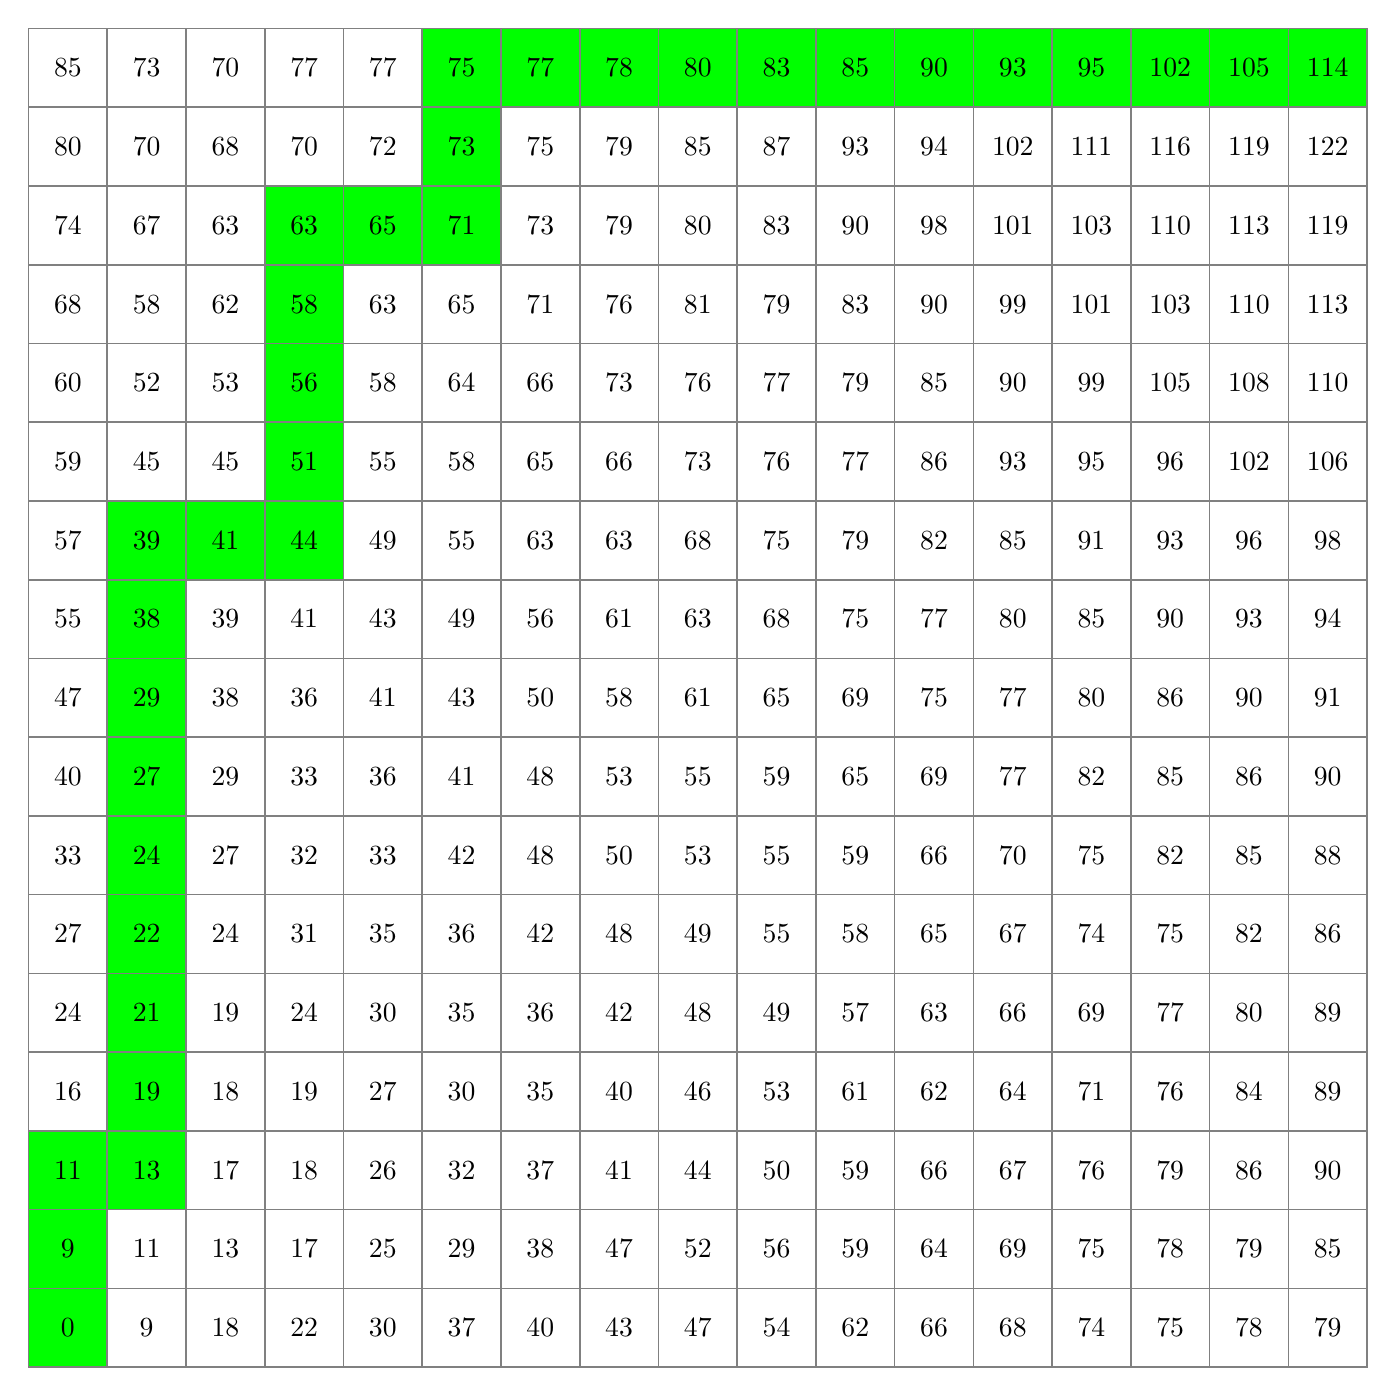
\begin{tikzpicture}[cell/.style = {rectangle,draw=gray,semithick,minimum size=1cm,outer sep=0mm}]
\node[cell,fill=blue!20] at (0,0) {};
\node[cell,fill=red!20] at (16,16) {};
\visible<2>{\foreach \j\i in 
{ 0/0,1/0,2/0,2/1,3/1,4/1,5/1,6/1,7/1,8/1,9/1,10/1,10/2,10/3,11/3,12/3,13/3,14/3,14/4,14/5,15/5,16/5,16/6,16/7,16/8,16/9,16/10,16/11,16/12,16/13,16/14,16/15,16/16 }
 \node[cell,fill=green] at (\i, \j) {};}
\foreach \i [count=\j from 0] in {0,9,18,22,30,37,40,43,47,54,62,66,68,74,75,78,79} \node[cell] at (\j, 0) {$\i$};
\foreach \i [count=\j from 0] in {9,11,13,17,25,29,38,47,52,56,59,64,69,75,78,79,85} \node[cell] at (\j, 1) {$\i$};
\foreach \i [count=\j from 0] in {11,13,17,18,26,32,37,41,44,50,59,66,67,76,79,86,90} \node[cell] at (\j, 2) {$\i$};
\foreach \i [count=\j from 0] in {16,19,18,19,27,30,35,40,46,53,61,62,64,71,76,84,89} \node[cell] at (\j, 3) {$\i$};
\foreach \i [count=\j from 0] in {24,21,19,24,30,35,36,42,48,49,57,63,66,69,77,80,89} \node[cell] at (\j, 4) {$\i$};
\foreach \i [count=\j from 0] in {27,22,24,31,35,36,42,48,49,55,58,65,67,74,75,82,86} \node[cell] at (\j, 5) {$\i$};
\foreach \i [count=\j from 0] in {33,24,27,32,33,42,48,50,53,55,59,66,70,75,82,85,88} \node[cell] at (\j, 6) {$\i$};
\foreach \i [count=\j from 0] in {40,27,29,33,36,41,48,53,55,59,65,69,77,82,85,86,90} \node[cell] at (\j, 7) {$\i$};
\foreach \i [count=\j from 0] in {47,29,38,36,41,43,50,58,61,65,69,75,77,80,86,90,91} \node[cell] at (\j, 8) {$\i$};
\foreach \i [count=\j from 0] in {55,38,39,41,43,49,56,61,63,68,75,77,80,85,90,93,94} \node[cell] at (\j, 9) {$\i$};
\foreach \i [count=\j from 0] in {57,39,41,44,49,55,63,63,68,75,79,82,85,91,93,96,98} \node[cell] at (\j, 10) {$\i$};
\foreach \i [count=\j from 0] in {59,45,45,51,55,58,65,66,73,76,77,86,93,95,96,102,106} \node[cell] at (\j, 11) {$\i$};
\foreach \i [count=\j from 0] in {60,52,53,56,58,64,66,73,76,77,79,85,90,99,105,108,110} \node[cell] at (\j, 12) {$\i$};
\foreach \i [count=\j from 0] in {68,58,62,58,63,65,71,76,81,79,83,90,99,101,103,110,113} \node[cell] at (\j, 13) {$\i$};
\foreach \i [count=\j from 0] in {74,67,63,63,65,71,73,79,80,83,90,98,101,103,110,113,119} \node[cell] at (\j, 14) {$\i$};
\foreach \i [count=\j from 0] in {80,70,68,70,72,73,75,79,85,87,93,94,102,111,116,119,122} \node[cell] at (\j, 15) {$\i$};
\foreach \i [count=\j from 0] in {85,73,70,77,77,75,77,78,80,83,85,90,93,95,102,105,114} \node[cell] at (\j, 16) {$\i$};
\end{tikzpicture}
}
\end{center}
\end{frame}

\begin{frame}[fragile]{ここまでの振り返り}{アルゴリズム=自明または「前処理$\to$相似問題$\to$後処理」}

{
%\fontsize{9}{10}\selectfont
\begin{tabular}[h]{r l}
\CL スペースシャトル & $T(n) = () + T(n-1) + T(n-1) + (+)$ \\
\CL 飛行船  & $T(n) = () + T(n-1) + T(n-1) + (+)$ \\
\CL 一方向最短経路 & $T(n) = () + T(n-1) + T(n-1) + (min)$ \\
\CL 最短経路表示 & $T(n) = (if文) + T(n-1) + (画面出力)$ \\
\end{tabular}
}

\vfill
{
%\fontsize{9}{10}\selectfont
\begin{tabular}[h]{r l}
\CL スペースシャトル & 整列(特にマージソート)と同類 \\
\CL 飛行船 & 整列(特にマージソート)と同類 \\
\CL 一方向最短時間 & 整列(特にマージソート)と同類 \\
\CL 最短経路表示 & 探索(特に二分探索)と同類 \\
\end{tabular}
}

\end{frame}

\begin{frame}[fragile]{問題2.0}{}
各点の重みが以下で与えられたとして\textcolor{blue}{A=(j=2,i=5)}から\textcolor{red}{B=(j=13,i=13)}への最短距離を求めよ。
各点は4近傍(4連結)である。

\begin{center}
\scalebox{0.3}{
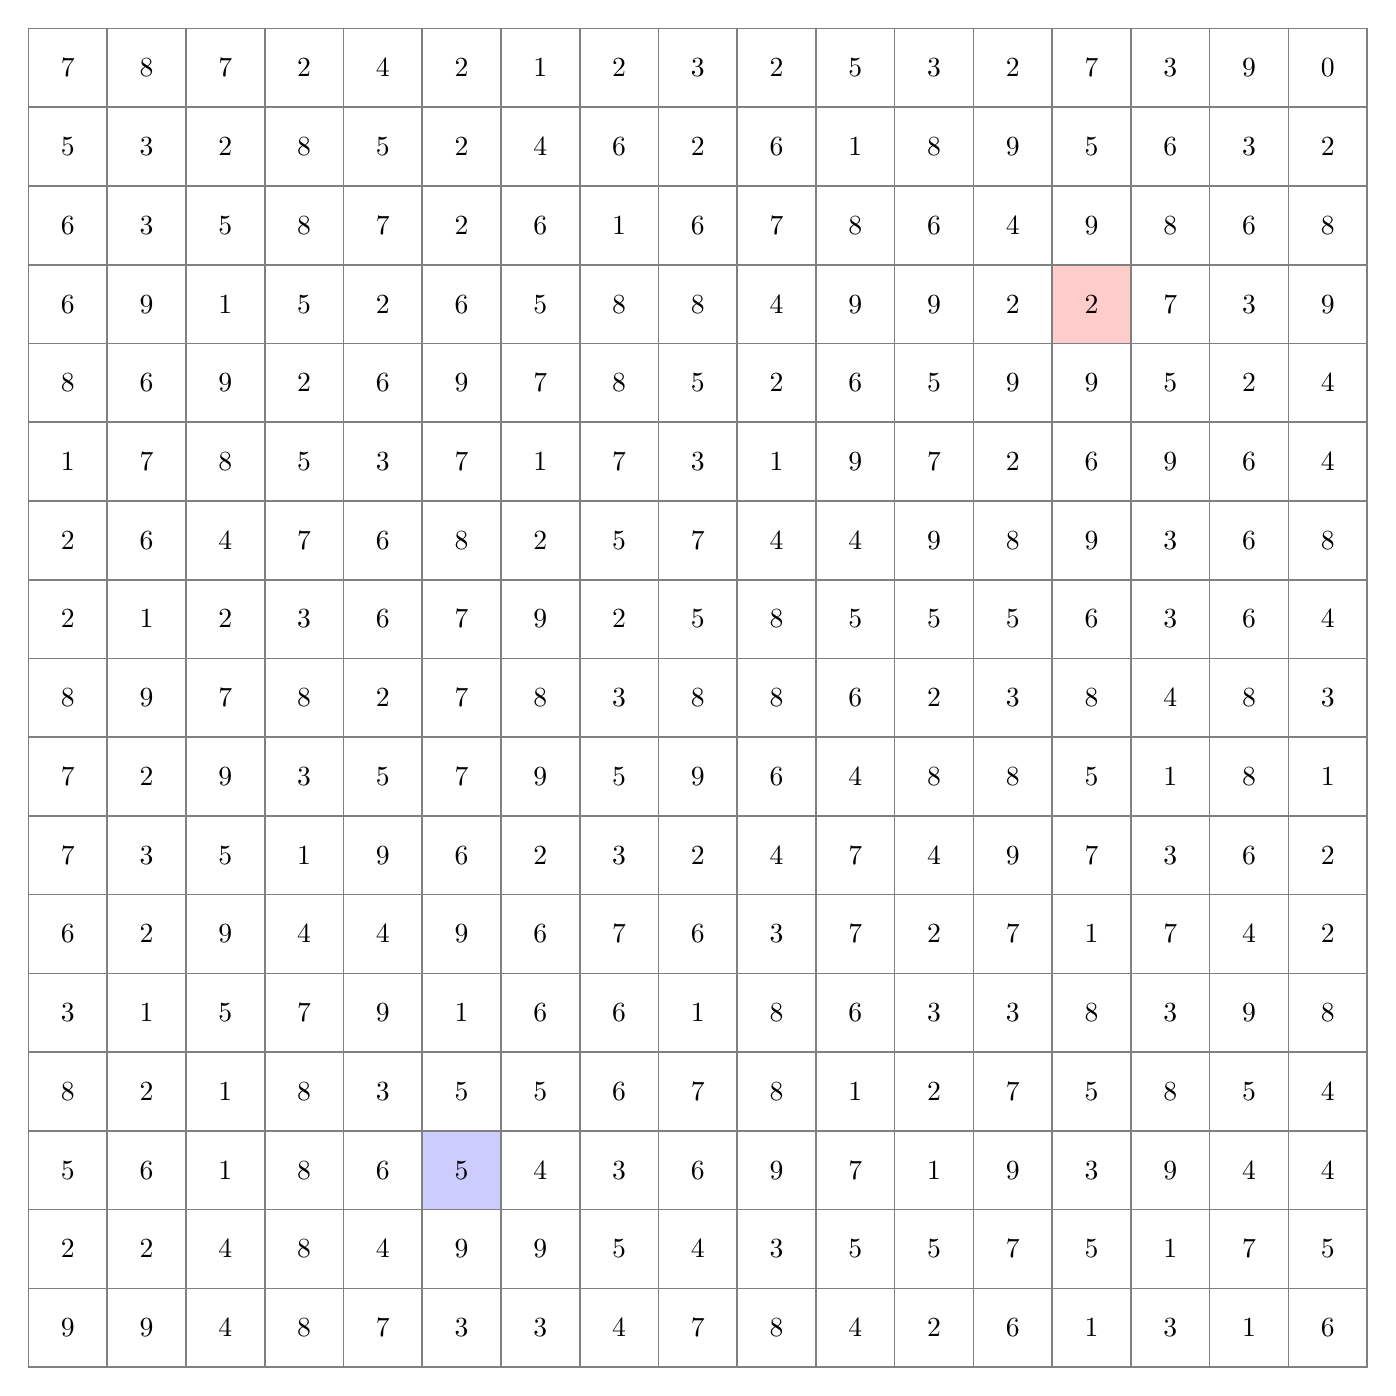
\begin{tikzpicture}[cell/.style = {rectangle,draw=gray,semithick,minimum size=1cm,outer sep=0mm}]
\node[cell,fill=blue!20] at (5,2) {};
\node[cell,fill=red!20] at (13,13) {};
    \foreach \i [count=\j from 0] in {9,9,4,8,7,3,3,4,7,8,4,2,6,1,3,1,6} \node[cell] at (\j, 0) {$\i$};
    \foreach \i [count=\j from 0] in {2,2,4,8,4,9,9,5,4,3,5,5,7,5,1,7,5} \node[cell] at (\j, 1) {$\i$};
    \foreach \i [count=\j from 0] in {5,6,1,8,6,5,4,3,6,9,7,1,9,3,9,4,4} \node[cell] at (\j, 2) {$\i$};
    \foreach \i [count=\j from 0] in {8,2,1,8,3,5,5,6,7,8,1,2,7,5,8,5,4} \node[cell] at (\j, 3) {$\i$};
    \foreach \i [count=\j from 0] in {3,1,5,7,9,1,6,6,1,8,6,3,3,8,3,9,8} \node[cell] at (\j, 4) {$\i$};
    \foreach \i [count=\j from 0] in {6,2,9,4,4,9,6,7,6,3,7,2,7,1,7,4,2} \node[cell] at (\j, 5) {$\i$};
    \foreach \i [count=\j from 0] in {7,3,5,1,9,6,2,3,2,4,7,4,9,7,3,6,2} \node[cell] at (\j, 6) {$\i$};
    \foreach \i [count=\j from 0] in {7,2,9,3,5,7,9,5,9,6,4,8,8,5,1,8,1} \node[cell] at (\j, 7) {$\i$};
    \foreach \i [count=\j from 0] in {8,9,7,8,2,7,8,3,8,8,6,2,3,8,4,8,3} \node[cell] at (\j, 8) {$\i$};
    \foreach \i [count=\j from 0] in {2,1,2,3,6,7,9,2,5,8,5,5,5,6,3,6,4} \node[cell] at (\j, 9) {$\i$};
    \foreach \i [count=\j from 0] in {2,6,4,7,6,8,2,5,7,4,4,9,8,9,3,6,8} \node[cell] at (\j, 10) {$\i$};
    \foreach \i [count=\j from 0] in {1,7,8,5,3,7,1,7,3,1,9,7,2,6,9,6,4} \node[cell] at (\j, 11) {$\i$};
    \foreach \i [count=\j from 0] in {8,6,9,2,6,9,7,8,5,2,6,5,9,9,5,2,4} \node[cell] at (\j, 12) {$\i$};
    \foreach \i [count=\j from 0] in {6,9,1,5,2,6,5,8,8,4,9,9,2,2,7,3,9} \node[cell] at (\j, 13) {$\i$};
    \foreach \i [count=\j from 0] in {6,3,5,8,7,2,6,1,6,7,8,6,4,9,8,6,8} \node[cell] at (\j, 14) {$\i$};
    \foreach \i [count=\j from 0] in {5,3,2,8,5,2,4,6,2,6,1,8,9,5,6,3,2} \node[cell] at (\j, 15) {$\i$};
    \foreach \i [count=\j from 0] in {7,8,7,2,4,2,1,2,3,2,5,3,2,7,3,9,0} \node[cell] at (\j, 16) {$\i$};
\end{tikzpicture}
}
\end{center}
\end{frame}

\begin{frame}[fragile]{}{}
帰納法の前提が崩れている:Aを求めるためにBを求めるためにAが必要
\vfill
検索→ダイクストラ法(Dijkstra's algorithm)

https://ja.wikipedia.org/wiki/ダイクストラ法

\vfill
名前だけでも覚えて帰るのか、丸暗記するのか
\end{frame}

\begin{frame}[fragile]{}{}
\begin{tabular}[h]{r l l}
\CL 線形探索 & \visible<2->{先頭を選択} & \visible<3->{実装簡単} \\
\CL 二分探索 & \visible<2->{真ん中を選択} & \visible<3->{実装簡単}\\
\CL バブルソート & \visible<2->{先頭を処理} & \visible<3->{実装簡単}\\
\CL クイックソート & \visible<2->{「順序化」分割} & \visible<3->{実装簡単}\\
\CL マージソート & \visible<2->{無条件分割、マージ} & \visible<3->{実装簡単}\\
\CL ダイクストラ & \visible<4->{三角不等式で選択} & \visible<5>{実装簡単}\\
\end{tabular}

\vfill
\begin{itemize}%\itemsep8pt
\item 別ものに見えるならアルゴリズムを覚えるのは大変
\item \visible<3->{プログラムは覚える価値がない}
\item \visible<3->{ビー玉の例えはわかるのだが、、、}
\item \visible<5>{まさか昨日実装することになろうとは}
\end{itemize}
\end{frame}

\begin{frame}[fragile]{}{}
\begin{itemize}\itemsep8pt
\item 解ける問題と解けない問題
\item 解ける問題と解けない問題と解ける問題に似た問題
\end{itemize}

\vfill
{\fontsize{4}{6}\selectfont
\begin{columns}[T]
\begin{column}{0.3\textwidth}
プログラミングコンテストチャレンジブック
\begin{markdown}
- 全探索(再帰、スタック、キュー)
- 貪欲法
- 動的計画法
- 木、グラフ,最短経路、最小全域木、ユークリッドの互除法
- 二分探索
- 尺取り法?
- ネットワークフロー、最小カット、被覆問題
- 計算幾何
- 分枝限定法(min-maxがない), A*, 文字列探索, 分割統治法
\end{markdown}
\end{column}
\begin{column}{0.3\textwidth}
プログラミングコンテスト攻略のためのアルゴリズムとデータ構造
\begin{markdown}
- ソートアルゴリズム
- データ構造:スタック、キュー、リスト
- 探索:線形、二分、ハッシュ
- 再帰と分割統治法
- 整列:マージ、クイック、計数ソート
- 木:二分木探索
- ヒープ
- 動的計画法
- グラフ:BFS, DFS
- 高度なデータ構造:お互いに素、トポロジカルソート、最小全域木、計算幾何
- 動的計画法、整数論、ヒューリスティック探索
\end{markdown}
\end{column}
\begin{column}{0.3\textwidth}
最強最速アルゴリズマー養成講座 プログラミングコンテストTopCoder攻略ガイド
\begin{markdown}
- 第4章 シミュレーション
- 第5章 全探索
- 第6章 計算量
- 第7章 動的計画法・メモ化
- 第8章 探索範囲を狭めるアルゴリズム
- 第9章 応用問題
- 第10章 グラフ問題対策
- 第11章 数学問題対策
\end{markdown}
\end{column}
\end{columns}
}
\end{frame}

\begin{frame}[fragile]{アルゴリズムの高速化}{}
\begin{itemize}\itemsep20pt
\item 今回アルゴリズムは考えたが、再帰関数で実装すると遅すぎて現実的ではない
\item 高速化が必要(その前に観察が必要)
\item 動的計画法に注目
\end{itemize}
\end{frame}

\end{document}
